\section{Examples}
\subsection{}

\begin{frame}[fragile]{Language discriminator}
    \begin{block}{}<+->
        Problem: given a word, discriminate it as English (0) vs.\ German (1)
    \end{block}

    \centering
    \begin{tikzpicture}[node distance=3mm, slstm/.style={lstm, font=\footnotesize, minimum height=5mm}]
    % Nodes.
    \node (lstm 00) [slstm] {LSTM};
    \node (lstm 10) [slstm, above=of lstm 00] {LSTM};

    \foreach \i in {1, ..., 4} {
        \pgfmathtruncatemacro{\j}{\i - 1}

        \foreach \layer in {0, 1} {
            \node (lstm \layer\i) [slstm, right=of lstm \layer\j] {LSTM};
        }
    }

    \foreach \layer in {0, 1} {
        \node (lstm \layer 5) [block, font=\footnotesize, right=of lstm \layer 4] {$\cdots$};
        \node (lstm \layer 6) [slstm, right=of lstm \layer 5] {LSTM};
    }

    \node (dense) [dense, minimum height=5mm, font=\footnotesize, above=of lstm 16] {dense};
    \node (sigmoid) [gate, minimum height=5mm, font=\footnotesize, right=of dense] {$\sigma$};
    \node (output) [font=\footnotesize, right=of sigmoid] {$[0, 1]$};

    \foreach \i/\char in {0/k, 1/o, 2/s, 3/t, 4/r, 5/$\cdots$, 6/<end>} {
        \node (input \i) [word, below=of lstm 0\i] {\texttt{\char}};
    }

    % Arrows.
    \foreach \i in {0, ..., 6} {
        \draw [path] (input \i) -- (lstm 0\i);
        \draw [path] (lstm 0\i) -- (lstm 1\i);
    }

    \foreach \i in {1, ..., 6} {
        \pgfmathtruncatemacro{\j}{\i - 1}

        \foreach \layer in {0, 1} {
            \draw [path] (lstm \layer\j) -- (lstm \layer \i);
        }
    }

    \draw [path] (lstm 16) -- (dense);
    \draw [path] (dense) -- (sigmoid);
    \draw [path] (sigmoid) -- (output);
\end{tikzpicture}

%%% Local Variables:
%%% mode: latex
%%% TeX-master: "../rnn"
%%% End:


    \begin{columns}
        \begin{column}{0.61\textwidth}
            \vspace{-5mm}
            \begin{itemize}
                \item LSTM state size = 128
                \pause
                \item Data: $10^4$ English \& German words
                \begin{itemize}
                    \item Max length: 14 characters
                    \item 80\%/20\% train/test split
                \end{itemize}
                \pause
                \item TensorFlow, 1 CPU \& 1 GPU:
                \begin{itemize}
                    \item $\sim$30~m to write code
                    \item 7~s to build model
                    \item 6~s to train 15 epochs
                \end{itemize}
            \end{itemize}
        \end{column}
        \begin{column}{0.39\textwidth}
            \pause
            Result: 81.9\% test accuracy
            \vspace{-17pt}
            \footnotesize
\begin{verbatim}
informatic: 0.083
helical: 0.050
lamentation: 0.097
baste: 0.528
surging: 0.222
kostritzer: 0.987
krombacher: 0.996
erhard: 0.272
wernesgruner: 0.992
oettingen: 0.794
\end{verbatim}
        \end{column}
    \end{columns}
\end{frame}

\setcounter{footnote}{0}

\begin{frame}{%
    Very short list of RNN applications\footnote{%
        Only one/a few representative papers cited because of space limitations.%
    } (1/2)%
}
    \begin{columns}
        \begin{column}{0.63\textwidth}
            \begin{itemize}[<+->]
                \item Speech-to-text \citep{Battenberg17}
                \item \bluelink{%
                    https://magenta.tensorflow.org/performance-rnn%
                }{%
                    Performance RNN%
                }: Google's music composer \citep{performanceRNN}
                \item Robotics control \citep{WuJIRS07}
                \item Handwriting-to-text \citep{GravesICASSP13}
            \end{itemize}
            \vspace{5mm}

            \visible<.->{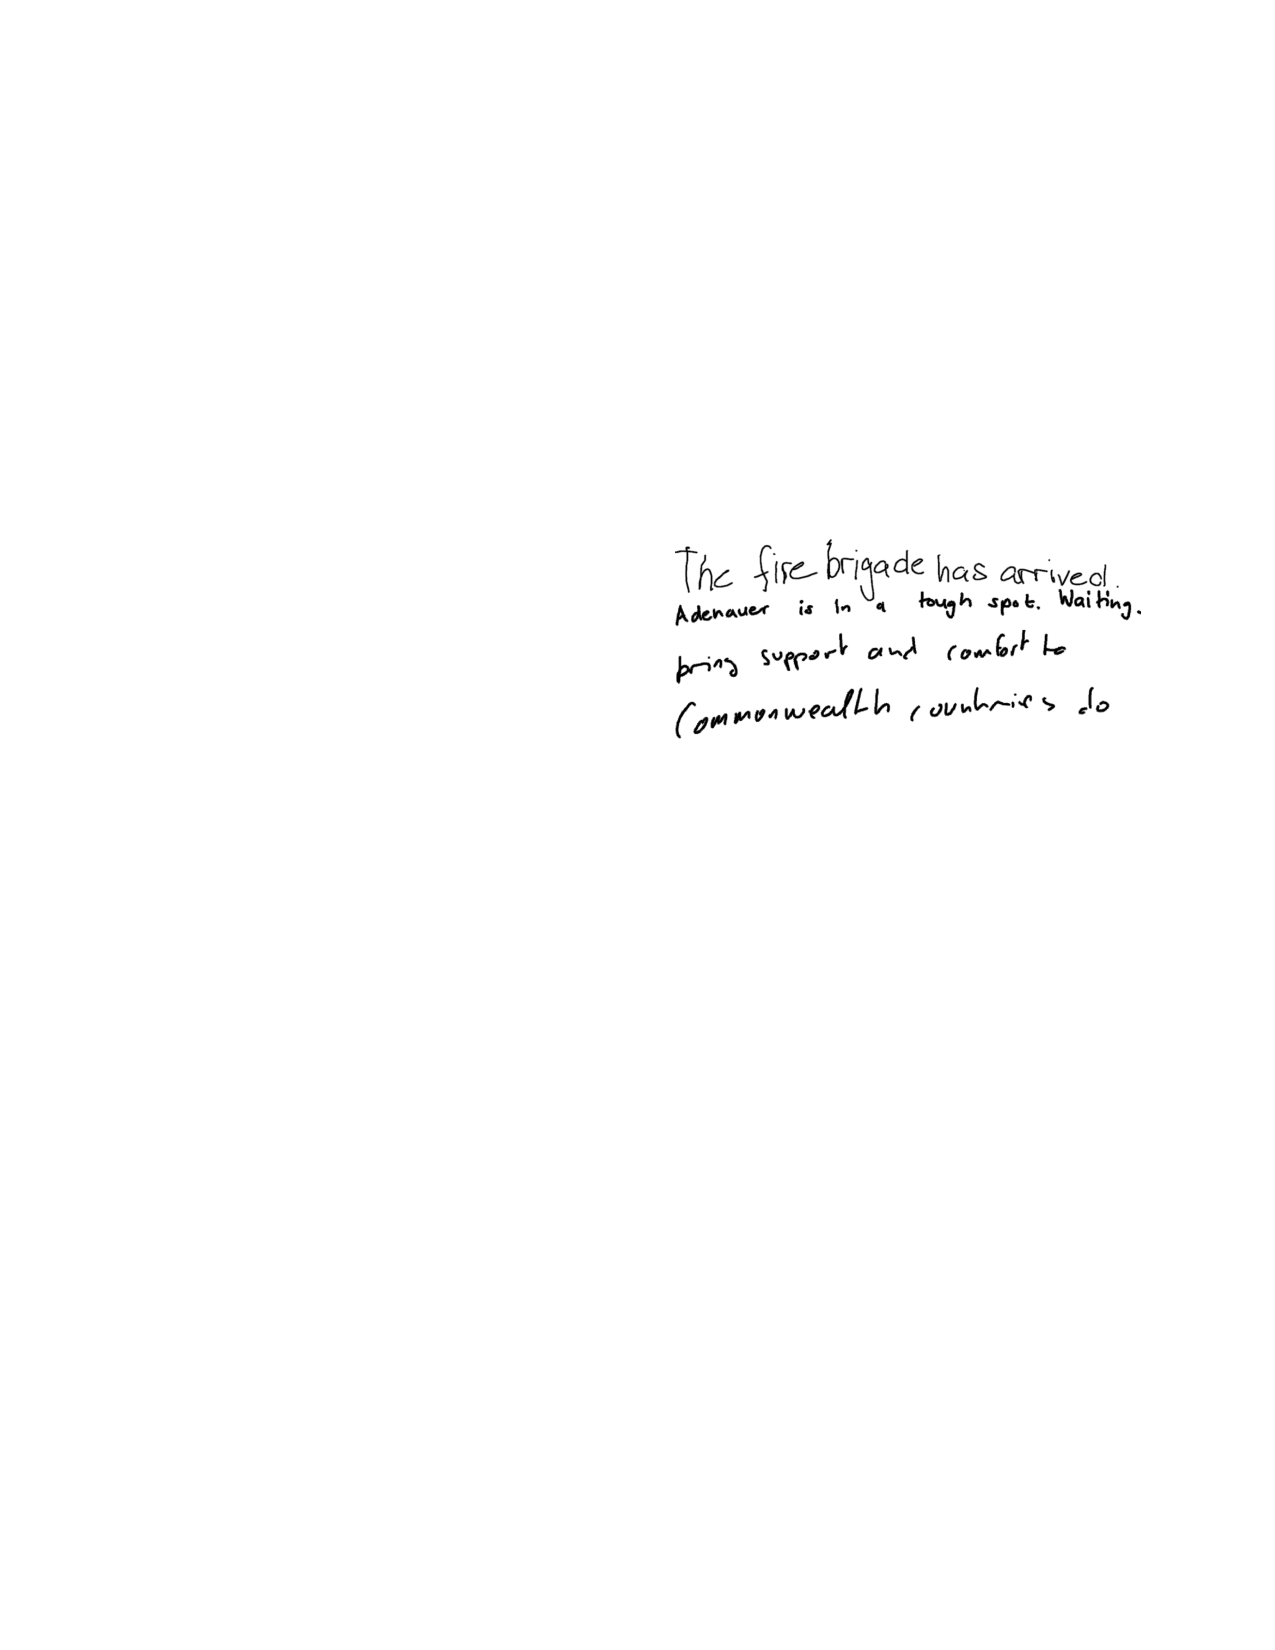
\includegraphics[width=\textwidth]{handwriting}}
        \end{column}
        \begin{column}{0.37\textwidth}
            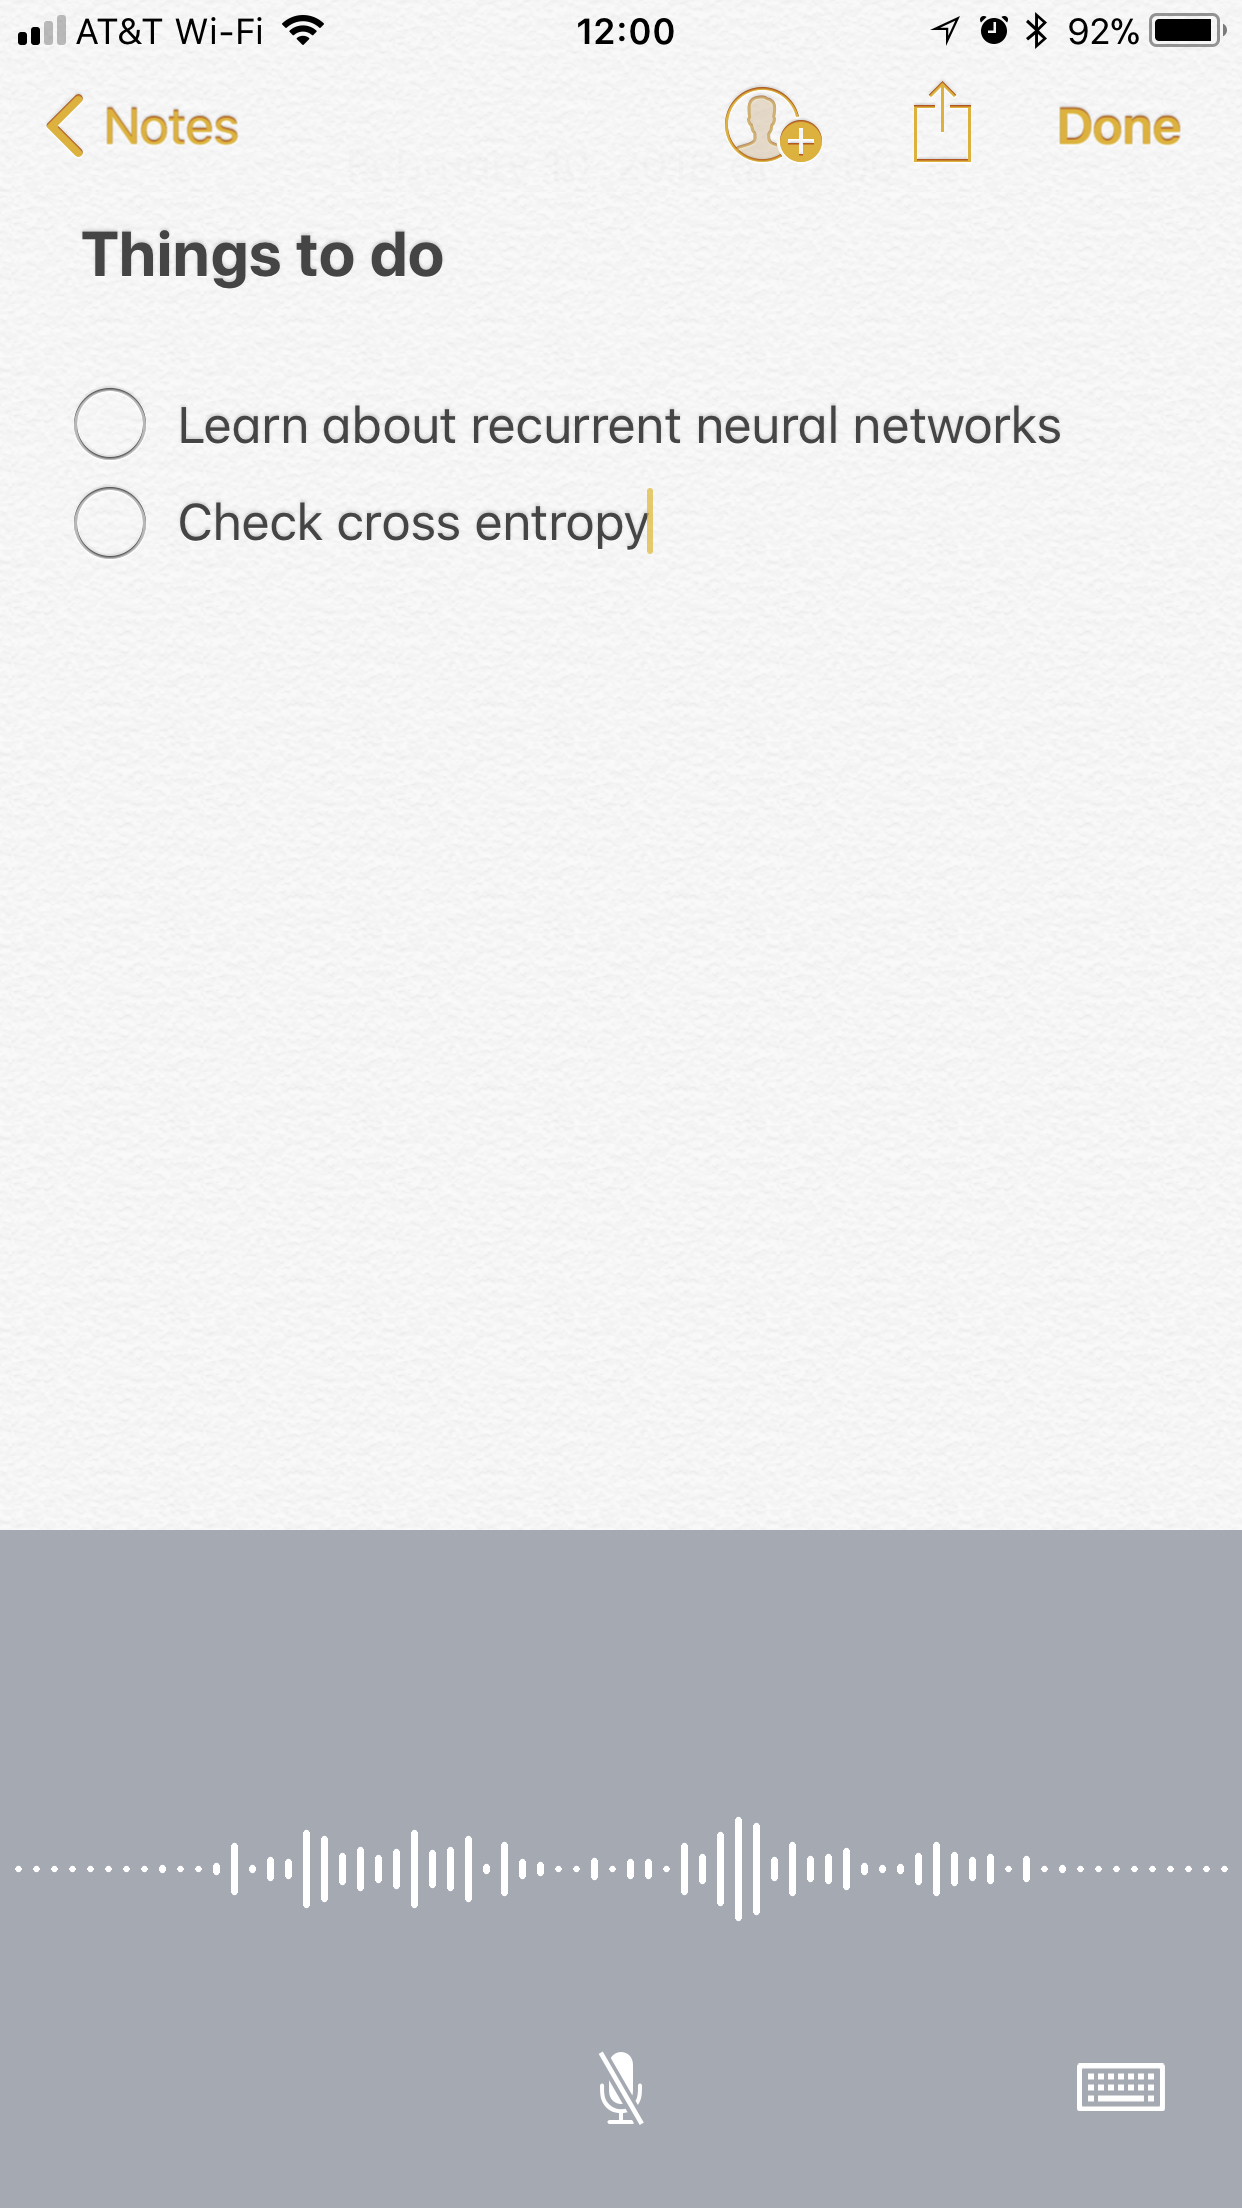
\includegraphics[width=\textwidth]{speech_text}
        \end{column}
    \end{columns}
    \vspace{2mm}
\end{frame}

\begin{frame}{Very short list of RNN applications (2/2)}
    \begin{itemize}[<+->]
        \item Given several video frames, predict the next frames
        \citep{SrivastavaICML15, Vukotic17}
    \end{itemize}
    \visible<.->{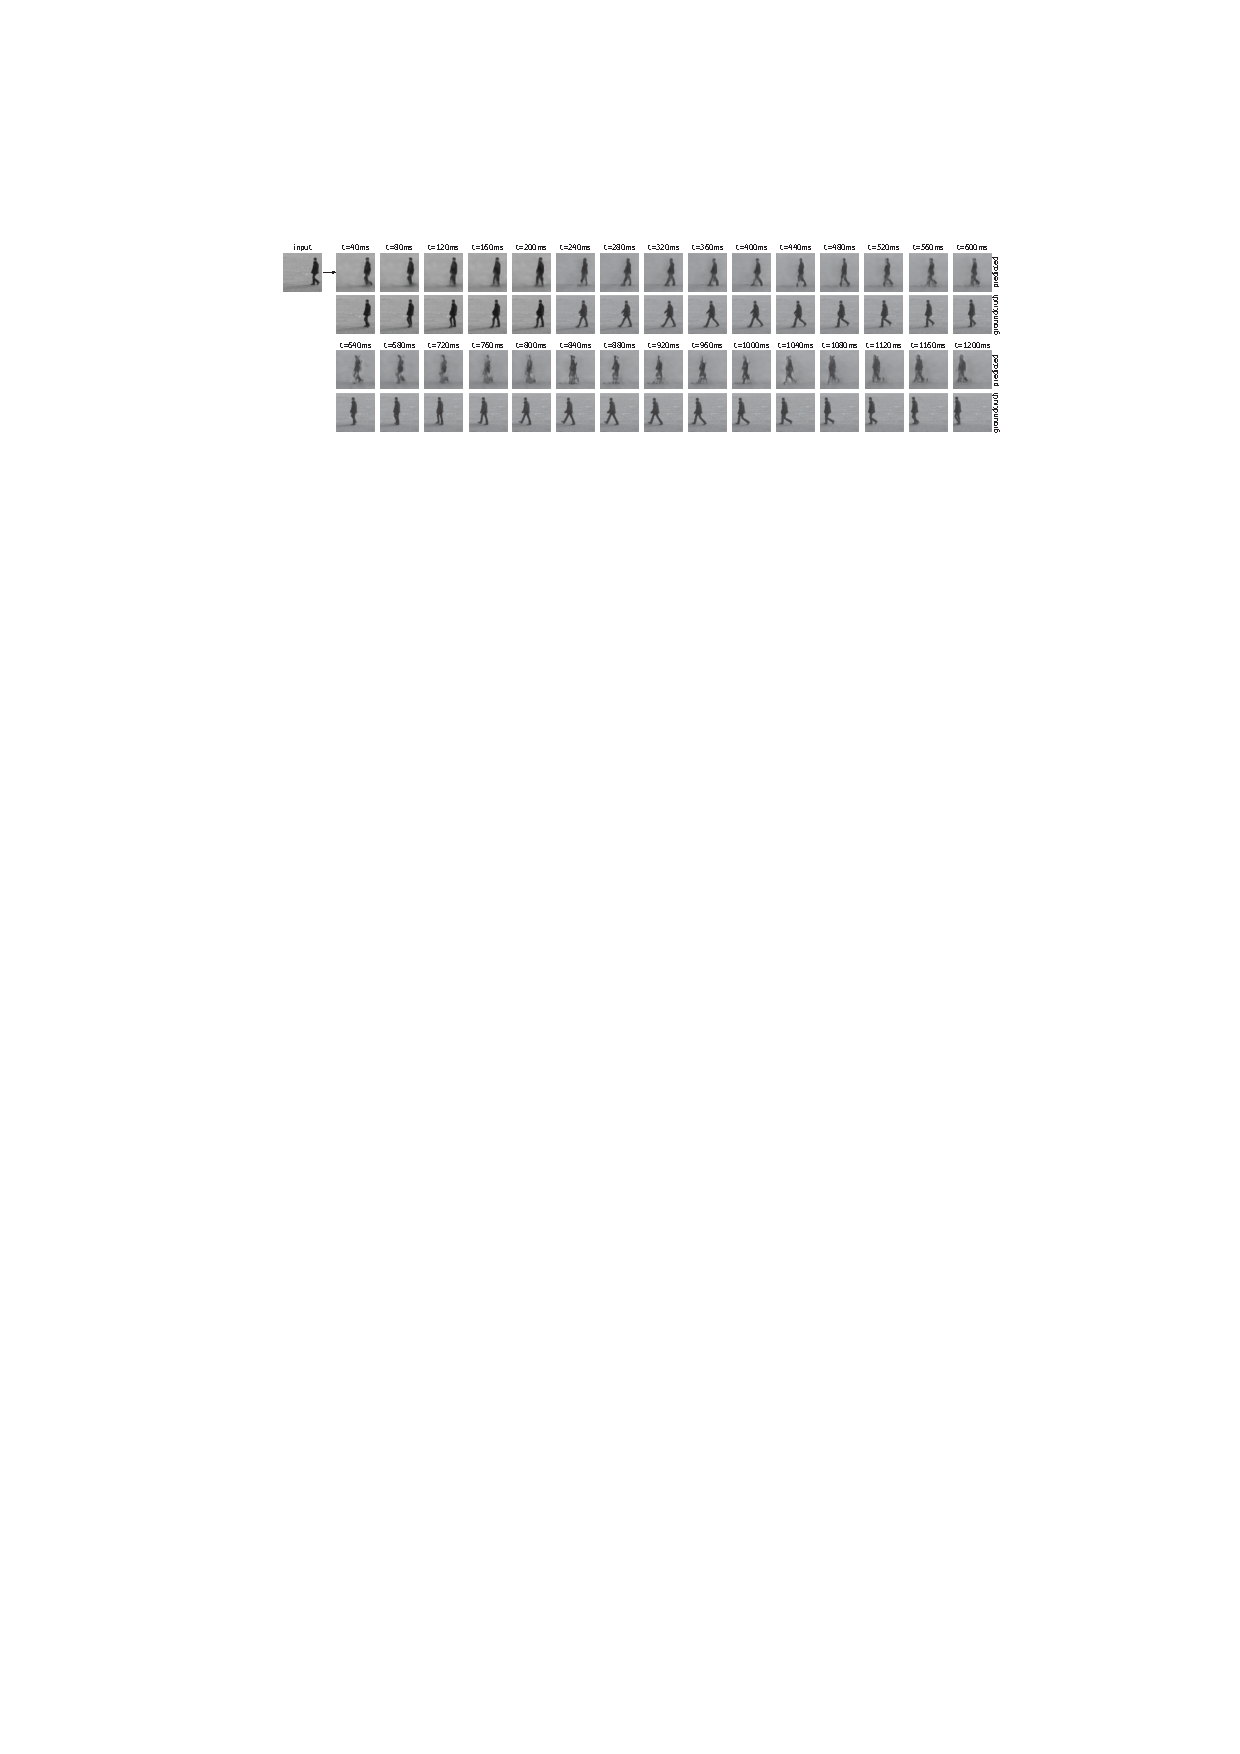
\includegraphics[width=\textwidth]{video_prediction}}

    \begin{columns}
        \begin{column}{0.43\textwidth}
            \begin{itemize}[<+->]
                \item Speaker attribution \citep{RenAAAICAI16}
                \item Modeling processes in physics (see \bluelink{https://dl4physicalsciences.github.io}{NIPS 2017 workshop on Deep Learning for Physical Sciences})
            \end{itemize}
        \end{column}
        \begin{column}{0.5\textwidth}
            \vspace{2mm}
            \visible<2->{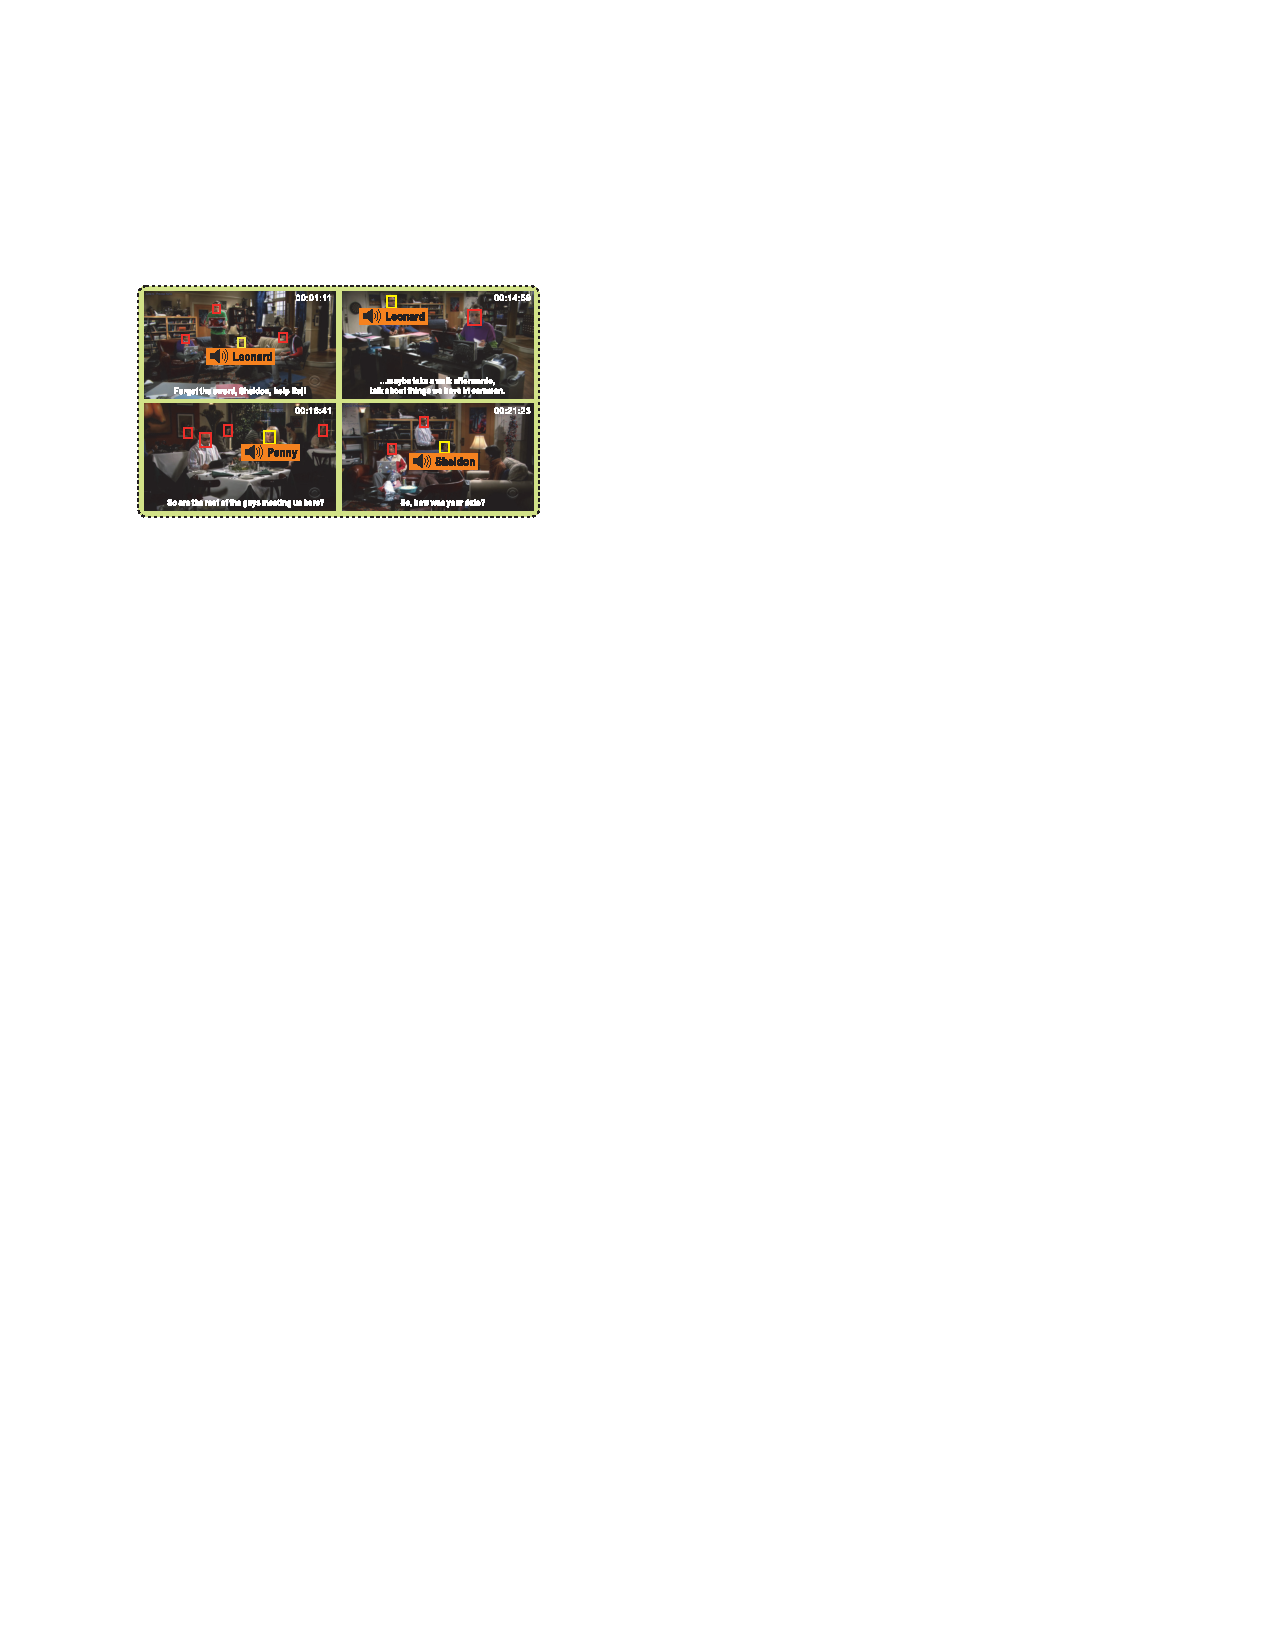
\includegraphics[width=\textwidth]{bigbang}}
        \end{column}
    \end{columns}
\end{frame}

%%% Local Variables:
%%% mode: latex
%%% TeX-master: "../rnn"
%%% End:
